\chapter{Design and Implementation}
\label{ch:design-implementation}

\section{Language and Machine Learning Framework}

% \begin{itemize}
%     \item Python as pre-existing machine learning frameworks
%     \item Tensorflow vs PyTorch (Tensorflow seemed nicer and more base code, first code seen for proof of concept was in tensorflow)
%     \item mutually exclusive due to CUDA implementations
% \end{itemize}

\subsection{Python}

When choosing a language to code this project in Python\footnote{\url{https://www.python.org}} was a clear choice. Whilst other languages offer better speed (C++\footnote{\url{https://cplusplus.com/}}, Rust\footnote{\url{https://www.rust-lang.org/}}), Python's advantage comes from its libraries.

Libraries are modular pieces of code written by other developers that can be integrated into a new piece of software to make common tasks easier. In Python, this is accomplished using the \verb|import| and \verb|from| syntax. Libraries vastly simplify coding as they can vastly reduce complex problems to simple functions. This is especially useful when dealing with complex machine learning functions, advanced mathematical algorithms such as Adam can be reduced to an import. Many Python libraries are written in lower-level languages like C or C++, allowing Python code to benefit from high performance while maintaining ease of use.

The vast majority of popular packages have a Python implementation that can be easily installed by the Python Package Index\footnote{\url{https://pypi.org/}}. Especially for machine learning, Python has some of the largest collections of relevant libraries of any language and is therefore the language of choice for this project.

\subsection{PyTorch versus TensorFlow}

There are many machine learning frameworks in Python, however, the primary two are PyTorch\cite{paszke2019pytorch} and TensorFlow\cite{abadi2016tensorflow}. They both offer nearly identical feature sets and performance so choosing between them is not a simple matter.

PyTorch was created by Meta in 2019. It is a lot newer and viewed as a more ``pythonic" framework\cite{chirodea2021comparison}. To be more ``pythonic" is to be more developer-friendlier by providing a simple interface to the library that developers already familiar with Python should easily pick up on. PyTorch supports a dynamic computation graph which enables dynamic changes of model architectures.

TensorFlow is a much more mature framework by Google released in 2015. It offers similar abstractions as PyTorch but is widely viewed to be slightly harder to develop in\cite{chirodea2021comparison}. TensorFlow uses an eager computation graph meaning no changes to model architectures can be made once a model is defined. Whilst this reduces flexibility during runtime, it allows for more optimisations to be made to the model architecture meaning greater accuracy, smaller model architectures, and sometimes quicker computations. TensorFlow also scales effectively running as efficiently as possible on desktop computers to large GPU clusters.

Unfortunately, TensorFlow and PyTorch are mutually exclusive. Both rely on separate versions of the CUDA backend to allow for GPU acceleration on NVIDIA architectures. Whilst this can be accomplished using virtually environments and other work arounds, it is generally recommended to use one or the other.

Due to their similarities, there is no clear choice between PyTorch and TensorFlow. Some trends have emerged, however, with PyTorch being used for research and development work where iterative improvements are desired whereas TensorFlow is employed for production environments. 

TensorFlow was chosen for this project for a number of reasons. Firstly, the flexibility that PyTorch offers is less important to this project as all models being used have had their architectures pre-defined. On the other hand, TensorFlow's ability to scale and optimise for the compute resources will be valuable for this project as it will be developed on smaller desktops but the final evaluation loops will be run on large GPU clusters. Furthermore, after trying out both TensorFlow and PyTorch, the author preferred the overall syntax of TensorFlow.

\section{Proof of Concept}
\label{sec:concept-design}

% \begin{itemize}
%     \item Re-use oriented design
%     \item Quick and dirty
%     \item test my theory
%     \item explain methodologies
% \end{itemize}

To validate whether blink-based DeepFake detection is resistant to adversarial noise, it was decided to construct a proof of concept during the Christmas holiday. As it is intended to be a small test-bed, small flaws in the design are acceptable. Therefore, it makes sense to use pre-existing models, solutions, and implementations where possible in order to speed up development.

The overall architecture of blink-based DeepFake detection is relatively simple. First, the landmarks around the face are computed to determine for every frame to generate an EAR-time graph. The graph can then be analysed to determine whether the video is real or not. 

\begin{algorithm}[h]
    \caption{Overall architecture of a blink-based DeepFake detector}
    \label{alg:blink-based}
    \begin{algorithmic}
        \Require video
        \State ears $\gets$ \{\}
        \For{frame $\in$ video}
            \State landmarks $\gets$ \textsc{GetLandmarks}(frame)
            \State ear $\gets$ \textsc{CalculateEAR}(landmarks) \Comment{If no landmarks, no value appended}
            \State \textsc{Append}(ears, ear)
        \EndFor
        \State classification $\gets$ \textsc{EARAnalysis}(ears)
    \end{algorithmic}
\end{algorithm}

It was decided to use an EAR-based approach over a custom blink model because it allows for complex analysis. EAR data is more precise than the binary open or close of a custom model, allowing for analysis of not just the frequency of blinks but more subtle details like how the blink starts and ends, the velocity of the eye, and whether the eye consistently returns to the same position when open. The flaws in EAR noted by Ictu Oculi\cite{li2018ictu} are valid but they rely on the eye landmarks being unreliably marked, with sufficiently advanced models trained with occlusions this can be overcome. 

To calculate the EAR, the six landmarks around the eye need to be located. Google's MediaPipe\cite{lugaresi2019mediapipe} was used for this purpose. It is designed to run in real-time on mobile devices and other edge computing resources and hence is very lightweight and fast. MediaPipe produces 478 landmarks in three dimensions that cover the entire face, a subset of twelve (six landmarks per eye) is then used to be the six landmarks for EAR. From the six landmarks, the EAR can be calculated using Equation \ref{eq:ear} and the average taken for the final EAR-time graph. If no landmarks can be detected for the frame, no EAR value is appended to the list. 

EAR analysis is performed using the hybrid of DeepVision\cite{jung2020deepvision} and Ictu Oculi\cite{li2018ictu} by counting the number of blinks in the EAR graph and comparing that to the human average. DeepVision's database was viewed as too time-consuming to produce and the simplicity of Ictu Oculi's approach was appealing for its speed advantage. In experiments, DeepVision's threshold of two standard deviations below the mean proved to be too inconsistent so a revised threshold of half a standard deviation above the minimum EAR value was chosen. The average human blinks 14 times per minute\cite{schiffman1990sensation}, DeepFakes will blink less than this and so if the subject of the video blinks less than 14 times a minute, the video is deemed as a fake. For an accurate classification, a minimum of 30 frames need to be in the final EAR list. If there are fewer values in the final list, the video classification of the video is unknown.

For traditional detectors, both ResNet and VGG architectures have been proven vulnerable to adversarial noise\cite{gandhi2020adversarial}. A ResNet-based DeepFake detector was implemented using an implementation from Tiwari\cite{tiwari2024deepfake}, a VGG-detector was implemented using a header from Krishna et al\cite{krishna2022deepfake} but the backbone was upgraded to VGG19 following research from Yadav et al\cite{yadav2024deepfake}. To extend frame-by-frame detection to entire videos, each frame in a video is analysed independently. If the frame is classified as fake then a counter is incremented by one. If the counter exceeds a given threshold (set as one hundred frames), the video is classed as fake.

Adversarial noise was added to images using the Foolbox library\cite{rauber2017foolbox}\cite{rauber2017foolboxnative}. FGSM was used as the method for noise due to its known effectiveness and speed\cite{gandhi2020adversarial}. $\epsilon$ was set to 0.1. To replicate real-life scenarios, noise was only added to faked videos and all models were solely trained on original videos, not noisy ones. This is because models would not be able to be trained on videos that have been manipulated by attacks specifically designed to disrupt the very model that is training. Only the VGG model is attacked during the proof of concept, with the ResNet model acting as a control model to show the effects of indirect noise on a model.

The models were trained on a subset of fifty real and fifty fake videos from the FaceForensics++ dataset\cite{dufour2019deepfakes}. Testing was run over a further fifty real and fifty fake videos. The results of the tests can be found in Section \ref{sec:concept-results}. FaceForensics++ was chosen as it was the most robust dataset available at the time. More have been tested in the main code. Hyperparameters for the VGG and ResNet models were left the same as the original implementations. To reduce overfitting, only one frame per second was extracted and used for training. To ensure a realistic test, no model is ever trained on images that have been injected with adversarial noise.

\section{Main DeepFake Detection Algorithm}

% \begin{itemize}
%     \item pseudocode of main algorithm
%     \item if at any point something fails, mark as fake (ensures resiliency)
%     \item emphasise each part is interchangeable
% \end{itemize}

The main DeepFake detection algorithm is similar to the one discussed in the proof of concept (Algorithm \ref{alg:blink-based}) in terms of structure. The code in the main algorithm is an alteration of the subroutine calls, making each subroutine return more accurate results. Other improvements were made such as general improving speed and modularity of the code. To further improve testing and evaluation, a number of different options for each component were developed as each section of the algorithm is interchangeable. 

To improve resiliency against adversarial noise attacks, the entire algorithm is fail negative. If any section of the algorithm were to fail then the video would be deemed a fake. For example, if no facial landmarks are detected in a frame, then the video is declared fake.

Whilst all of the separate components, such as facial landmarking models, are pre-existing neural networks, certain novel contributions have been made. The first is the use of univariate time series analysis of the EAR graph. This allows for more sophisticated and complex analysis to be done, which will hopefully allow for consistent and accurate classification. Furthermore, some of the facial landmarking models used had only been implemented in PyTorch, this project marks their first implementation using TensorFlow.

\subsection{Face cropping}
\label{sec:face-cropping}

One common feature across all DeepFake detection and facial landmarking models is that they perform best when the face being analysed fills the entire frame, because background information is often irrelevant and can disrupt the model. As such, it is useful to have a preprocessing step which crops a frame to just the faces in the frame, using a face detector model. 

One of the most efficient models available is YuNet\cite{wu2023yunet}. YuNet is designed to run in real-time (approximately 1 millisecond per frame) on a CPU, whilst retaining a high degree of accuracy. It only contains 75,856 parameters, with many models requiring fifty times more parameters to reach similar levels of accuracy. More parameters mean longer computation times, which was deemed unacceptable for a model designed to run on edge devices. With neural networks, quicker computation times often come at the expense of reduced accuracy; whilst this is still the case with YuNet, it still achieves ``similar accuracy to other small models" on standardised benchmarks. \verb|OpenCV| contains an implementation of YuNet for use in Python\cite{yunetpyton}.

A more accurate CNN for detecting faces is Multitask Cascaded Convolutional Networks (MTCNN)\cite{zhang2016joint}. MTCNN is more accurate, achieving 0.851 mean average precision on benchmarks, compared to YuNet's 0.836. The accuracy comes with a significant speed decrease. Where YuNet takes one millisecond per frame, MTCNN takes ten milliseconds. The \verb|mtcnn| library\cite{centeno2024mtcnn} is a popular Python implementation of MTCNN written in TensorFlow.

To attain the optimal combination of speed and accuracy both YuNet and MTCNN are used to identify faces in a video. An initial pass on all frames is done via YuNet, if no faces are found in a frame then MTCNN is used to identify the faces. To improve the performance of MTCNN, faces are processed in batches of 8. It was noted during testing that when exposed to adversarial noise, YuNet was prone to miss faces, as such the confidence YuNet required to mark a face was reduced from 0.9 to 0.7. Only the primary face in each frame is used, for the first frame this is taken as the face with the highest confidence from the model, for subsequent frames it is the face with the smallest Euclidean distance between the vertices of the bounding box. The process for cropping the face from a video is shown in Algorithm \ref{alg:face-detection}.

\begin{algorithm}[H]
    \caption{The method for cropping faces from a video}
    \label{alg:face-detection}
    \begin{algorithmic}
        \Require video
        \State faces\_per\_frame $\gets$ \{\}
        \For{frame $\in$ video}
            \State faces\_coords $\gets$ \textsc{Yunet}(frame)
            \If{faces\_coords $\neq$ \{\}}
                \State \textsc{Append}(faces\_per\_frame, face\_coords)
            \Else
                \State faces\_coords $\gets$ \textsc{MTCNN}(frame)
                \State \textsc{Append}(faces\_per\_frame, face\_coords) \Comment{Will deliberately append empty set if no faces}
            \EndIf
        \EndFor
        \State faces $\gets$ \{\}
        \State previous\_face $\gets$ \{\}
        \For{frame\_faces$\in$ faces\_per\_frame}
            \State best\_face $\gets$ \{\}
            \If{previous\_face $=$ \{\}}
                \State best\_face $\gets$ frame\_faces[0]
            \Else
                \State best\_face $\gets$ \textsc{MinimumDistance}(frame\_faces,previous\_face)
            \EndIf
            \State previous\_face $\gets$ best\_face
            \State \textsc{Append}(faces, best\_face)
        \EndFor
    \end{algorithmic}
\end{algorithm}

\subsection{Eye Landmark Detection}
\label{sec:eye-landmark}

% \begin{itemize}
%     \item EAR needs 6 points per eye so lets get them
%     \item Facial landmarking is a common superset problem
%     \item Introduce 68 landmarks and datasets
%     \item Most popular ones aren't viable as built to be small to fit in a package (dlib, opencv...) or to run on a phone (mediapipe)
% \end{itemize}

To determine the EAR in a specific frame, the six landmarks around each eye need to be located. There are a large number of Python packages which come with facial landmarking features, unfortunately most of these are unsuitable for use in a state-of-the-art detector as they are insufficiently accurate. The models included in packages are either compressed for ease of distribution or optimised to run on devices with reduced computational capabilities. Hence, a custom implementation of a pre-existing method is required.

\subsubsection{Weakly Supervised Eye Landmarks Detection}
\label{sec:sweld}

% \begin{itemize}
%     \item Looked promising
%     \item Most accurate according to landmarks in paper \& only model focussing specifically on eye landmarking
%     \item Has a ``good enough" implementation details
%     \item Had issues
%     \begin{itemize}
%         \item Landmarks from regions (mention other paper that managed it
%         \item difficulty implementing in tensorflow
%         \item after a month scrapped development
%     \end{itemize}
% \end{itemize}

The first method researched for eye landmark detection was Weakly Supervised Eye Landmarks Detection (WSELD)\cite{huang2020eye}. In facial landmarking benchmarks (Section \ref{sec:face-datasets}), WSELD is the most accurate with respect to eye landmarking when compared to current state-of-the-art methods on mean squared error loss.

A Regional-CNN (R-CNN)\cite{ren2015faster} outputs initial landmarks. R-CNNs are a special type of CNN that uses Region of Interest (ROI) to locate objects within an input so that later layers can specifically focus on those regions. R-CNN consists of three primary components, a traditional CNN backbone for feature extraction, a Region Proposal Network (RPN) which selects hypothetical areas of interest, a final ROI pooling layer that combines the features from the backbone with the regions to produce regions that can be used for future layers of the network. WSELD uses R-CNN to produce both eye-bounding box regions (the regions of interest) and initial predictions of eye landmarks.

To augment the initial eye landmarks to final, precise landmarks, WSELD employs a custom RNN. The primary component of the RNN is an LSTM module which uses the previous predictions to refine the current prediction. Dense layers surround the LSTM unit to adapt the input and output data into usable formats.

An overall network diagram is shown in Figure \ref{fig:wseld}.

\begin{figure}[h]
    \centering
    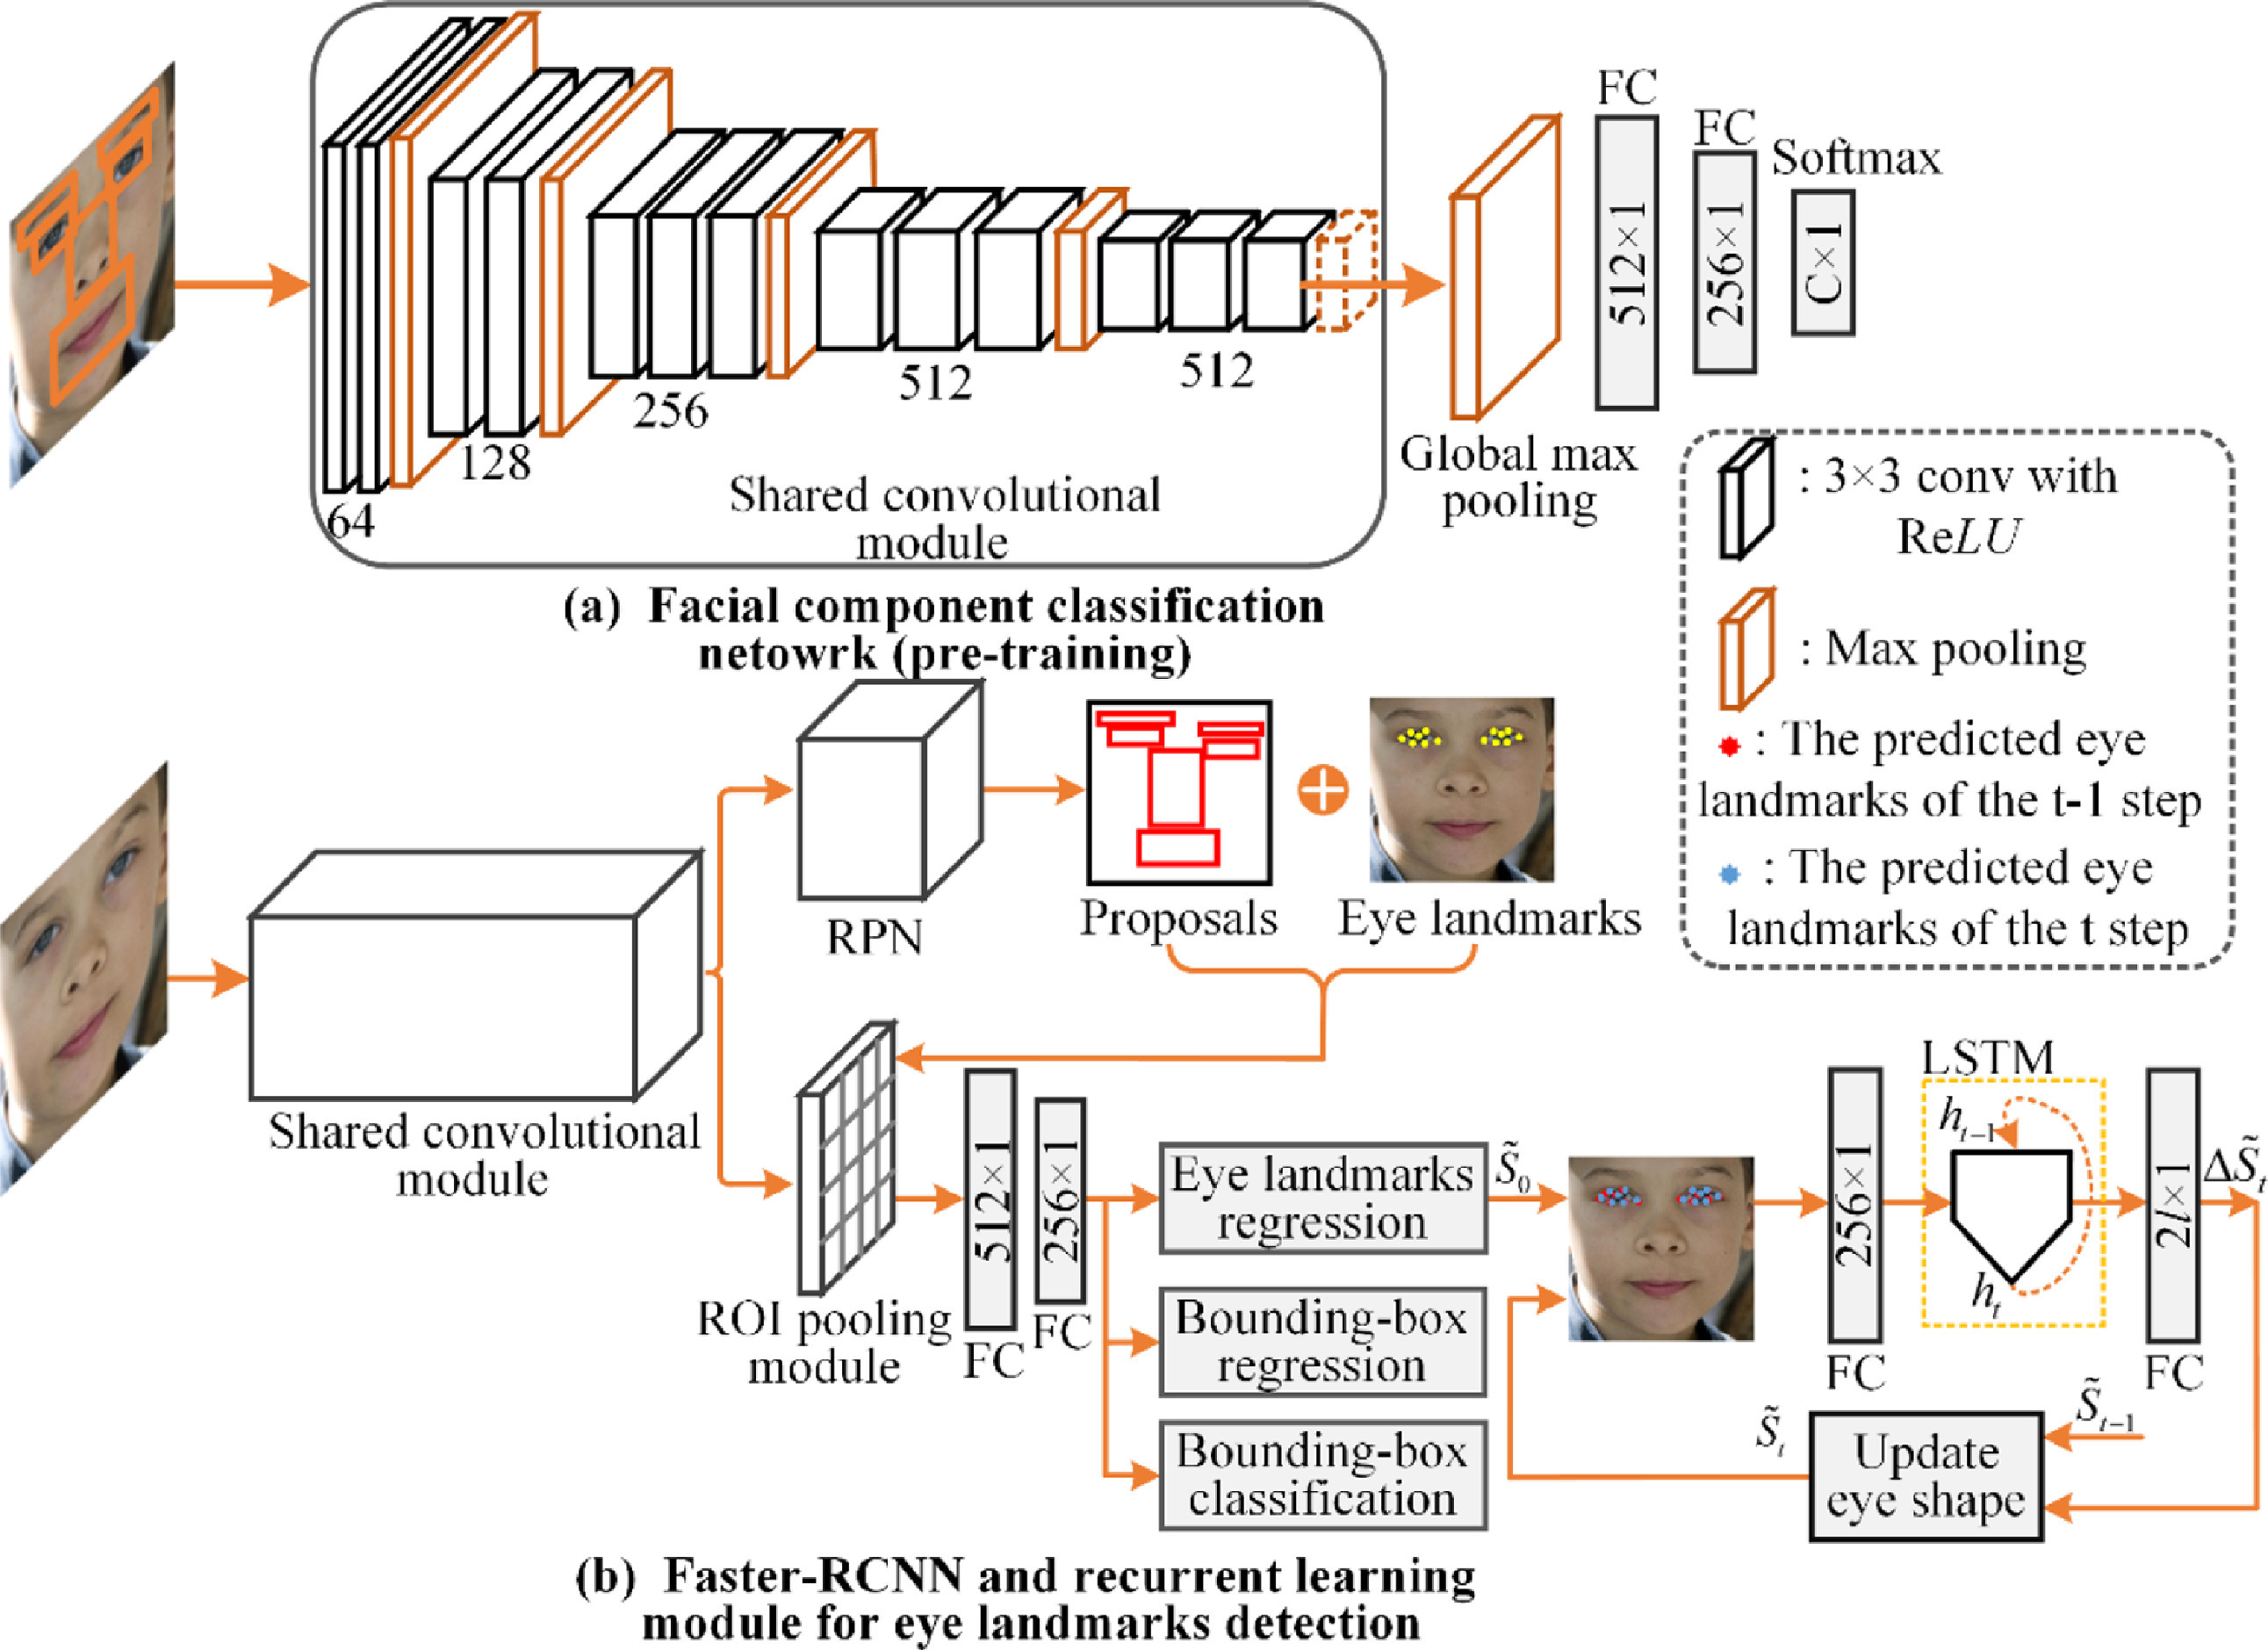
\includegraphics[width=0.75\linewidth]{dissertation//figures/wseld.jpg}
    \caption{Network diagram of WSELD\cite{huang2020eye}}
    \label{fig:wseld}
\end{figure}

Whilst the original paper gave clear implementations, their findings were difficult to replicate. No code was supplied with the paper so all code had to be created from scratch. The most confusing aspect of the model was generating landmarks from a RPN. As the name suggests, RPNs are only able to generate regions, as such it would seem to be impossible to generate landmarks. A similar paper was able to produce results on multiple facial regions\cite{tang2018facial} but, again, no code was provided. In this implementation, it was assumed a dense layer with the number of outputs equal to the number of landmarks was incorporated into the output of the RPN. Furthermore, this was the author's first time coding a substantial learning framework in TensorFlow. There is no pre-built RPN module so one needs to be created from scratch, a number of open source implementations exist\cite{hxuaj2021tensorflow2}\cite{kewar2021region} but these do not generate landmarks. It was attempted to create a custom R-CNN but there was a seeming constant stream of bugs. The bugs, along with there being no way to confirm whether the method of adding landmarks to RPN was successful, resulted in the development of WSELD being halted in favour of a new facial landmarking network.

\subsubsection{Pre-implemented Models}

% \begin{itemize}
%     \item Re-use oriented design
%     \item papers with code
%     \item Used best models which had pre-existing implementations (one for fast, one more accurate)
%     \item couldve optimised for 6 landmarks but didnt want to mess with model architectures that were known working (batch size probably meant nothing would change anyway)
% \end{itemize}

To avoid a repetition of the WSELD implementation, it was decided to switch to a reuse-oriented methodology for facial landmarking. For a model to be considered, it must have an open-source implementation available. PapersWithCode\footnote{\url{https://paperswithcode.com}} is an aggregation site which ranks models on popular machine-learning problems and links to known codebases where possible. 

Facial landmark detection is a common problem in machine learning. The vast majority of available training datasets (Section \ref{sec:face-datasets}) contain the six points required for EAR calculation and as such any model that can be trained on these datasets can be used for eye landmarking. In theory, it is possible to optimise the networks for solely eye landmark detection, however, this will not be done due to the potential that has to disrupt a network that is known to be working.

\subsubsection{High-Resolution Network}

% \begin{itemize}
%     \item modular sequences
%     \item keeps high resolution layers in context at all times
%     \item generic network but with a specific implementation for eye landmarking
%     \item Heatmap per landmark
% \end{itemize}

The most implemented facial landmark detector on PapersWithCode is High-Resolution Network (HRNet)\cite{sun2019high}. HRNet is a proposal for a novel architecture of CNNs that has applications in many fields and one of those fields is facial landmarking.

HRNet's novel contribution is CNNs working in parallel. Typical CNNs have one layer following another, whilst HRNet contains multiple CNNs working at a different resolution over the image. Similar to a CNN, the network gradually introduces lower and lower resolution layers to focus on more generic features, but, at all times, keeps the higher resolution layers in context which can refine their feature predictions based on the input from lower-level feature predictions. Lower-resolution layers are connected to higher-resolution layers through fusion layers which either upsample or downsample the feature predictions using either a CNN for downsampling or a bilinear for upsampling. An overview of the architecture for an HRNet is shown in Figure \ref{fig:hrnet-diagram}.

\begin{figure}[h]
    \centering
    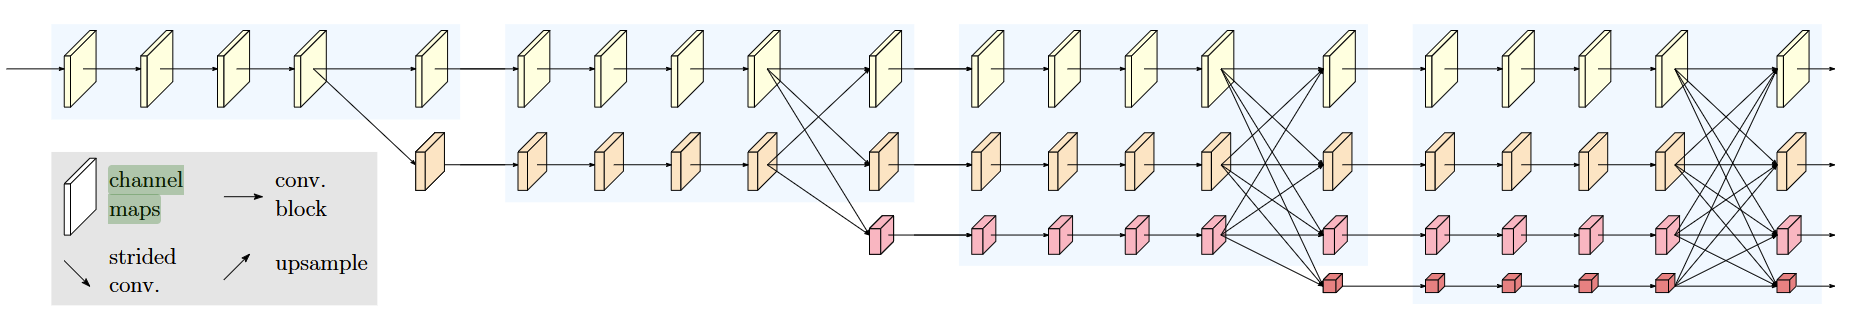
\includegraphics[width=1\linewidth]{dissertation//figures/hrnet-network.png}
    \caption{A generic network diagram for a HRNet\cite{sun2019high}}
    \label{fig:hrnet-diagram}
\end{figure}

Whilst HRNet is a generic architecture, it has been applied with great effect to facial landmarking. Such an implementation has been made open source in HRNet's official GitHub repository\cite{zhao2019facial} which details the specific architecture of HRNet uses for facial landmarking. Similar to Figure \ref{fig:hrnet-diagram}, the network consists of four distinct modules, with each module containing four convolutional layers. Each module introduces one additional parallel network. Each layer consists of 18, 36, 72, and 144 filters respectively.

Instead of a set of coordinates for landmarks, the output of HRNet is a heatmap of the likely locations of a landmark with the peak of the heatmap being the most probable location (Figure \ref{fig:hrnet-output}). As such, the location of the maximal value of the heatmap can be taken as the final location of a landmark. Whilst a simple version would be to simply take the index of the maximal value in the array, this neglects the possibility of the landmark being in the subpixel domain. The output heatmap is relatively low resolution ($64\times64$), so it is highly likely that the peak is within a subpixel. The problem has been research by Fisher et al.\cite{fisher1996comparison}. The most accurate algorithm proposed is Centre of Mass 7 (CoM7) which assumes the heatmap follows a Gaussian distribution and can therefore be estimated using a weighted average as shown through Equation \ref{eq:com7}. Firstly, the coordinates of the maximal value are computed and stored as $x,y$. Six values on either side of the maximal value are retrieved ($f(x)$). The original equation assumes one dimension, but it can be expanded to two by performing the calculation twice, one for $x$ and one for $y$.

\begin{figure}[H]
    \centering
    \begin{subfigure}{0.25\textwidth}
        \centering
        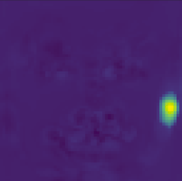
\includegraphics[width=\textwidth]{dissertation/figures/hrnet-single.png}
        \caption{The heatmap for a single landmark}
        \label{fig:hrnet-single}
    \end{subfigure}
    \hspace{3cm}
    \begin{subfigure}{0.25\textwidth}
        \centering
        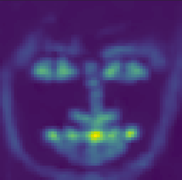
\includegraphics[width=\textwidth]{dissertation/figures/hrnet-multiple.png}
        \caption{The heatmap for all facial landmarks}
        \label{fig:hrnet-multiple}
    \end{subfigure}
    \caption{The heatmap outputs of HRNet}
    \label{fig:hrnet-output}
\end{figure}

\begin{equation}
    \label{eq:com7}
    \hat{x} = \frac{3f(x+3)+2f(x+2)+f(x+1)-f(x-1)-2f(x-2)-3f(x-3)}{f(x+3)+f(x+2)+f(x+1)+f(x)+f(x-1)+f(x-2)+f(x-3)}
\end{equation}

HRNet achieves state-of-the-art performance on facial landmarking datasets. It is currently ranked in the top 25 on a variety of datasets by the PapersWithCode\cite{paperswithcodehrnet}. As multiple CNNs are working in parallel, HRNet is often slower than a CNN on equivalent tasks. When trained, HRNet operates at approximately 30 frames per second when run on an RTX3060ti. As such, HRNet is not viable for real-time computation on edge devices but can be used for detection on powerful machines.

When training, the ground truth heatmap was generated by centring Gaussian noise with a $\sigma=1.5$ on the true landmark, all other values in the heatmap were set to 0. Following the HRNet code\cite{zhao2019facial}, each heatmap was $64\times64$. To align with the inputs for all the other models used in this project, the input was scaled up from $112\times112$ to $256\times256$. The model was trained for 60 epochs with mean squared error as the loss and the Adam\cite{kingma2014adam} optimiser.

\subsubsection{Practical Facial Landmark Detector}

% \begin{itemize}
%     \item speedy boi
%     \item uses mobilenet-techniques to reduce the size and increase the speed
%     \item still accurate tho
%     \item secret sauce is custom loss function
% \end{itemize}

A Practical Facial Landmark Detector (PFLD)\cite{guo2019pfld} is an accurate landmarker that is primarily designed for speed. Developed to run on edge devices such as phones, the model can achieve speeds of 150 frames per second on some phones with a minimal reduction in accuracy.

The architecture of PFLD is more similar to a traditional CNN: a backbone that leads into a number of dense layers which produce the final classification. PFLD uses the MobileNet backbone\cite{howard2017mobilenets} for feature extraction. As discussed in Section \ref{sec:traditional-cnns}, MobileNet reduced the number of parameters in a network whilst retaining similar accuracy. While EfficientNet then scales up its network in response, PFLD keeps the reduced model size to allow it to run with reduced compute times. MobileNet also comes with a width hyperparameter that can further narrow down a network, increasing speed at the expense of accuracy. For this project, accuracy is more important than speed so only the most accurate MobileNet model is used, as such the width parameter is set to $1\times$. 

PFLD also includes an auxiliary network that is only used for training. To improve accuracy in a small network, PFLD uses a custom loss function which requires the pitch, yaw, and roll of a face. Whilst these could be calculated from the landmarks produced by the PFLD network, during the early stages, this is very inaccurate and can cause the model learning to stall. The auxiliary network picks up from an intermediary layer midway through the main backbone and outputs three values which are the predicted pitch, yaw, roll of the face.

The overall main backbone is taken from the PyTorch implementation\cite{zhao2019pfld} but with a header from a TensorFlow fork\cite{qi2019pfld} to align with the number of facial landmarks required.

\begin{figure}[H]
    \centering
    \begin{subfigure}{\textwidth}
        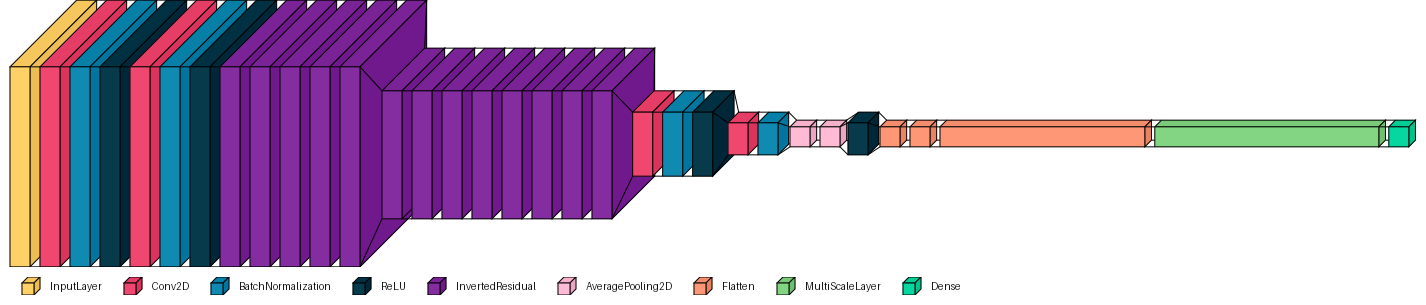
\includegraphics[width=\linewidth]{dissertation//figures/PFLD.png}
        \caption{The network diagram for PFLD}
    \end{subfigure}
    \begin{subfigure}{\textwidth}
        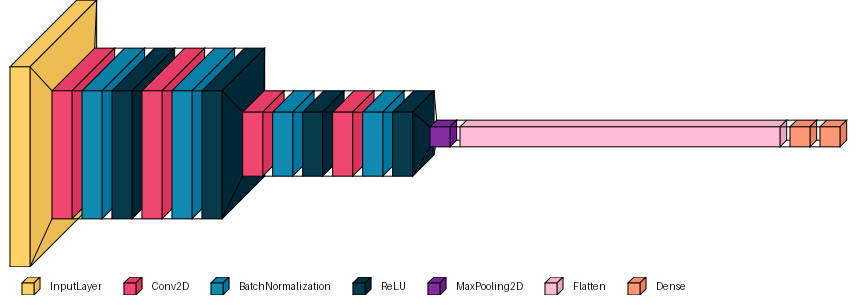
\includegraphics[width=\linewidth]{dissertation/figures/AuxiliaryNet.png}
        \caption{The network diagram for PFLD's auxiliary network}
    \end{subfigure}
    \caption{Network Architecture of PFLD (Generated using visualkeras\cite{Gavrikov2020VisualKeras})}
    \label{fig:pfld}
\end{figure}
One of the key contributions to PFLD's accuracy is a custom loss function. A typical facial landmarking model will use some form of distance metric for the loss function. These can only be done in two dimensions, neglecting geometric and structural information. For example, the more you turn your head relative to a camera, the closer your eyes will appear to the camera despite them remaining the same distance apart in three-dimensional space. Whilst large-scale models can get away with using conventional loss functions and brute force their way the inconsistencies, smaller models cannot. To take into account geometrical information, PFLD uses the pitch, yaw, and roll of a face from the auxiliary network to compute the following loss function:

\begin{equation}
    L =\sum^N_{n=1}\left(\sum^C_{c=1}\omega^c_n\sum^K_{k=1}(1-\cos{\theta^k_n})\right) ||d_n||^2_2
\end{equation}

$n$ represents the $n^\text{th}$ of $N$ landmarks. $C$ and $\omega$ are weighting parameters to equalise datasets. The dataset is divided into $C$ classes. A number of classes are proposed, but these require augmenting the dataset with hand labelled, as this is an individual project and some facial landmark datasets contain over 10,000 images (Section \ref{sec:face-datasets}) these weights are omitted to save time. The primary weighting parameters are $\theta^1, \theta^2,\theta^3$ which represent the difference the difference between the estimated and truth pitch, yaw, and roll respectively. As the delta goes up, so does the penalisation allowing the model to compensate for large deviations in head poses. Finally, L2 loss ($||d_n||^2_2$) is used as the primary loss component that is then weighted by the previous factors. 

To find the ground truth angles of the face, the Perspective-n-Point algorithm\cite{mallick2016head}\cite{hou2018face} maps sample points in three dimensions to two dimensions on the face, from which the facial angles can be calculated. The model was trained for 500 epochs following the PyTorch implementation\cite{zhang2016joint} using the Adam\cite{kingma2014adam} optimiser.

\subsubsection{Choice of Model}

Both models offer their own advantages and disadvantages. PFLD offers a much faster model, at the expense of accuracy, whereas HRNet offers accuracy at the expense of speed. The difference in accuracy is only expressed in the literature comparing them on the AFLW\cite{koestinger2011annotated}, where PFLD has a normalised mean error (NME) of 1.88 versus HRNet with 1.57. These are exceptionally close as most state-of-the-art models achieve an NME of 1.5-2\footnote{\url{https://paperswithcode.com/sota/facial-landmark-detection-on-aflw-full}}. As such, both models will be tested over the course of this project. If preference is required, due to time constraints, HRNet will be used as accuracy over speed is the priority for this project. Figure \ref{fig:eye-comparison} shows HRNet and PFLD landmarking the frame. HRNet is more accurate, landmarking the coordinates precisely. PFLD is less accurate often landmarking sections of the lower eyelid rather than the eye itself. However, these landmarks are still accurate in comparison to each other, the entire eye is simply translated down. As such, the EAR will not be affected and so PFLD can still be used effectively.

Furthermore, it is believed that slight inaccuracies in landmark detection will be consistent across the entire EAR graph, as such the various EAR analysis models should be able to learn the idiocracies of each model and compensate for them.

\begin{figure}[H]
    \centering
    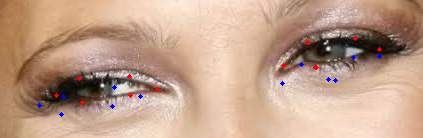
\includegraphics[width=0.5\linewidth]{dissertation//figures/compare_landmarks.png}
    \caption{A comparison of HRNet's (red) and PFLD's (blue) predictions}
    \label{fig:eye-comparison}
\end{figure}

\subsubsection{Facial Landmark Datasets}
\label{sec:face-datasets}

% \begin{itemize}
%     \item 68 landmarks (upsampling and downsampling where necessary)
%     \item list all of them and give brief overview
%     \item didnt use aflw due to inaccurate landmarks or not enough landmarks
%     \item reflected to double size
% \end{itemize}

Similar to DeepFake detection (Section \ref{sec:datasets}), large numbers of faces have been pulled from the internet and hand-labelled to enable the training and comparison of accurate facial landmarking models. The precise number of landmarks varies but the standard is 68 with some datasets labelling more landmarks, acting as a superset. 68 landmarks were used for this project as only the six eye landmarks for calculating the EAR are useful and the 68 landmarks are the smallest standardised size that covers all of them. Reducing the number of outputs significantly speeds up the model as fewer nodes are required to be trained. Where a model used more than 68 landmarks, a mapping was made from the model's landmarks to the main 68 and the rest of the landmarks were discarded.

\begin{figure}[h]
    \centering
    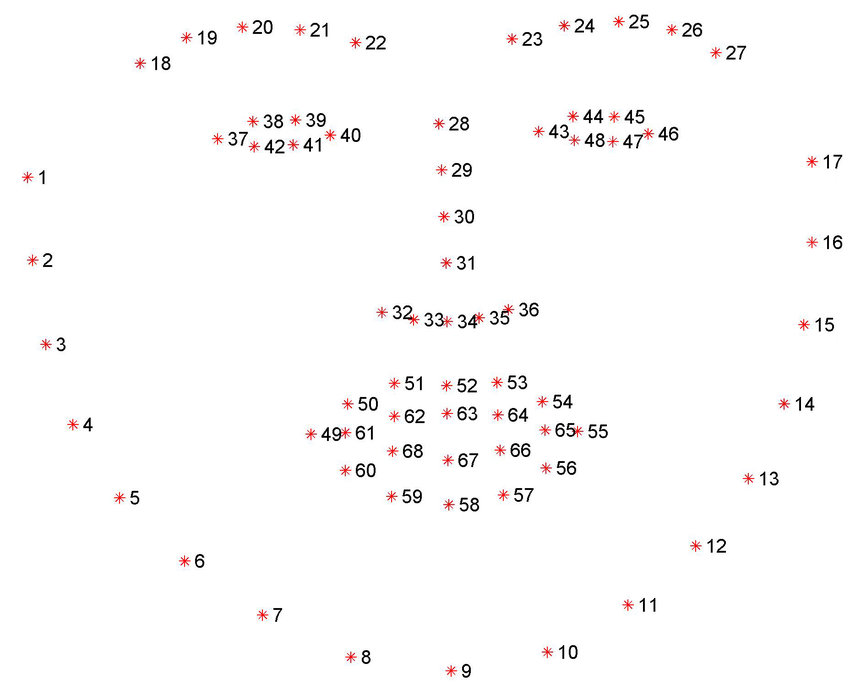
\includegraphics[width=0.5\linewidth]{dissertation//figures/facial-landmarks.jpg}
    \caption{The 68 facial landmarks common in facial landmarking datasets\cite{sagonas2016300}}
    \label{fig:facial-landarks}
\end{figure}

A variety of datasets were chosen with the primary aim to include a wide variety of facial poses, environmental factors, and occlusions. Increasing the variety of data allows for the model to learn in more challenging scenarios and hopefully become more robust.

The following datasets were used: 300W\cite{sagonas2016300}\cite{sagonas2013300}\cite{sagonas2013semi}, Labelled Face Parts in the Wild (LFPW)\cite{belhumeur2013localizing}\cite{mondal2021lfpw}, Caltech Occluded Faces in the Wild (COFW)\cite{burgos2022caltech}, Annotated Faces in the Wild\cite{zhu2012face}, HELEN\cite{le2012interactive}, and Wider Facial Landmarks in the Wild (WFLW)\cite{wayne2018lab}.

In total, these contain 11,495 labelled images. A common method of augmenting the dataset is to flip the images horizontally, which increases the dataset to 22,990 images. Data is scraped from a variety of imaging sites such as Flickr\footnote{\url{https://www.flickr.com/}}, Google\footnote{\url{https://images.google.co.uk/}}, and Yahoo!\footnote{\url{https://images.search.yahoo.com/}}. The dataset is very comprehensive covering a wide variety of individual characteristics like age, gender, and race. Environmental factors are also covered such as lighting, whether the photo was taken outside or inside. 

Two datasets (COFW and WFLW) were specifically chosen for their coverage of facial occlusions. Occlusions are where certain landmarks are obstructed from the view of the camera; for example, sunglasses blocking eyes and hair obscuring one side of the face. Some examples of occlusions are shown in Figure \ref{fig:occlusions}.

\begin{figure}[h]
    \centering
    \begin{subfigure}{0.45\textwidth}
        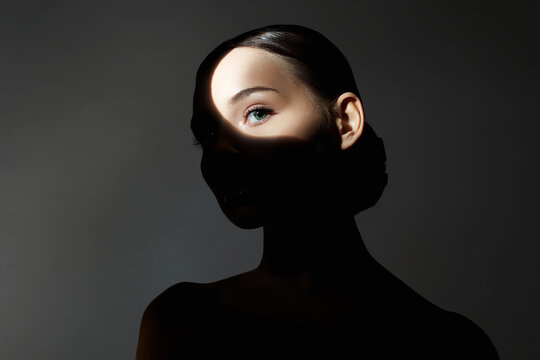
\includegraphics[width=1\linewidth]{dissertation//figures/shadow.jpg}
        \caption{A face occluded by shadow}
        \label{fig:occlusion-shadow}
    \end{subfigure}
    \hfill
    \begin{subfigure}{0.45\textwidth}
        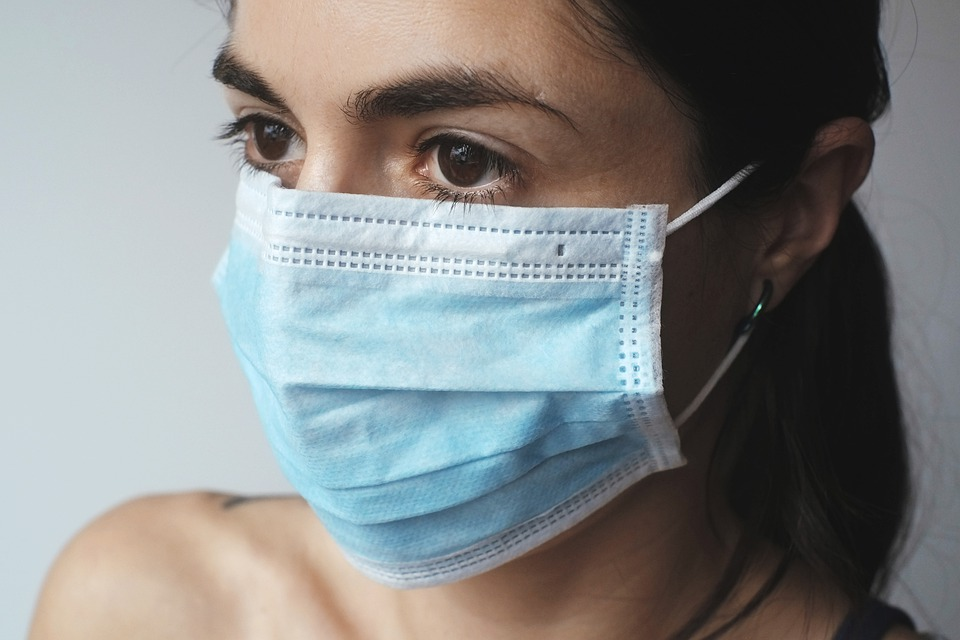
\includegraphics[width=1\linewidth]{dissertation//figures/occlusion-mask.jpg}
        \caption{A face occluded by a mask}
        \label{fig:occlusion:mask}
    \end{subfigure}
    \caption{Faces that have been partially occluded}
    \label{fig:occlusions}
\end{figure}

As explained in Section \ref{sec:face-cropping}, landmarking models benefit from faces filling the majority of images. To account for this, when training, the images are cropped to the facial region. This region is defined as the area bounded by the ground truth eye landmarks with 2\% padding on each side.

\subsection{Eye Aspect Ratio Analysis}

% \begin{itemize}
%     \item Can be abstracted to a univariate time series
%     \item Well researched
%     \item Classical methods exists (pyts library)
%     \item explain each one and give simple summary (1 paragraph)
%     \item As do deep learning frameworks (the other papers)
%     \item model diagrams for each one (maybe give a rough explanation as to the aims each one is doing?)
% \end{itemize}

With the eye landmarks located and the EAR calculated for each frame, the result is an EAR-time graph (Figure \ref{fig:sample-ears}). Existing blink-based DeepFake detectors will extract features from the graph such as frequency and period. A novel approach from this project is to use the entire EAR graph for analysis by abstracting the problem into univariate time series classification.

\begin{figure}[H]
    \centering
    \begin{subfigure}{0.45\linewidth}
        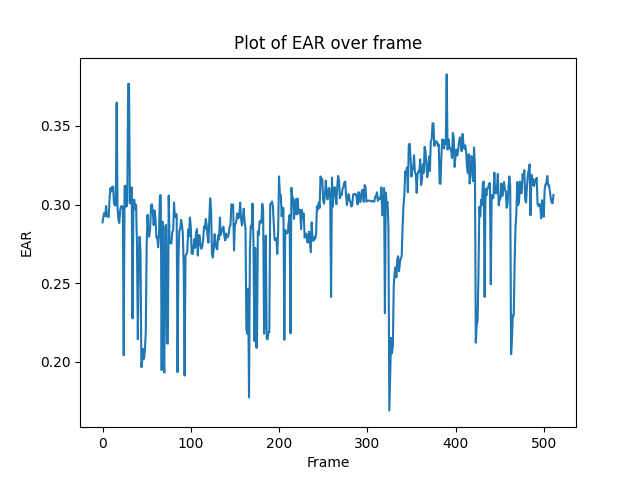
\includegraphics[width=\textwidth]{dissertation/figures/real-ear.png}
        \caption{The plot of a real EAR graph}
        \label{fig:real-ear}
    \end{subfigure}
    \begin{subfigure}{0.45\linewidth}
        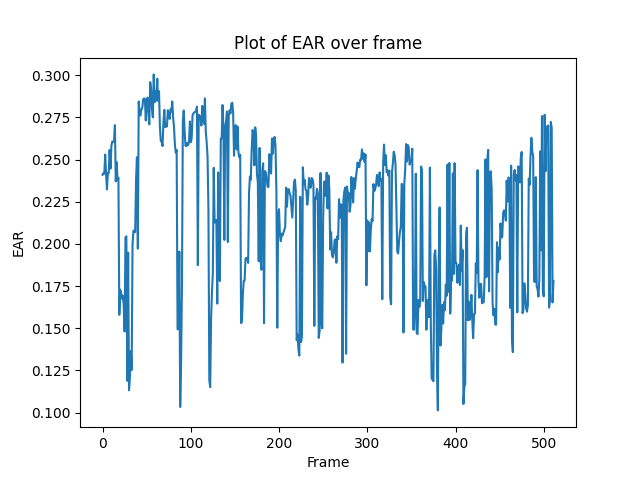
\includegraphics[width=\textwidth]{dissertation/figures/fake-ear.png}
        \caption{The plot of a fake EAR graph}
        \label{gif:fake-ear}
    \end{subfigure}
    \caption{Plots of sample EAR graphs}
    \label{fig:sample-ears}
\end{figure}

A univariate time series is a single point of data that varies over time. A large amount of research has been done into time series due to their frequent appearance in statistical models. Traditionally machine learning models struggle with temporal structures seen in time series but over time reliable methods have been developed. A comprehensive overview of sate-of-the-art time series algorithms for time series classification has been provided by Johann Faouzi\cite{faouzi2024time}.

Figure \ref{fig:sample-ears} shows how much a fake EAR graph differs compared to a fake graph. The real EAR plot has clear distinct blinks and a relatively consistent EAR when the eye is open. On the other hand, the fake EAR graph has a lot more noise an variation. The graph is almost constantly varying with no clear distinction between blinks and the eye being open and there is a lot more overall noise in the graph as a whole. As there are clear differences between a real EAR graph and a fake one, time series analysis should be able to successfully classify the two.

\subsubsection{K-Nearest Neighbours with Dynamic Time Warping}

K-Nearest Neighbours (k-NN) is a common algorithm for classification problems. Known training data is plotted in $n$-dimensional space where $n$ is the number of points of data. A new piece of data is classified by plotting it in the same space and determining which points it is ``nearest". The $k$ nearest neighbours' classification is checked and the majority classification is set as the classification for the new point. The metric for how ``near" one point is to another is a hyperparameter along with the value of $k$.

Euclidean distance is the most common algorithm for k-NN classifiers\cite{faouzi2024time} but it cannot be readily applied to time series. Each point in the time series would be compared independently by Euclidean distance which would throw away valuable temporal data. For example, with speech recognition where one sentence is spoken slower than another, the two time series would represent the same data but be far apart via Euclidean distance due to the time discrepancy.

The common solution is Dynamic Time Warping\cite{sakoe1978dynamic}. DTW is programmatically defined in Algorithm \ref{alg:dtw}. A cost matrix is computed which has the dimensions of the two time series being compared. For every value in the matrix, the cost is computed as the squared delta of the two values. A warped path is then constructed through the matrix starting at 0,0 and ending in the opposite corner. This path is constructed as the path that has minimum cost across the matrix whilst only moving towards the goal. The total cost of the path is the sum of all the cells it crosses through. The problem can be optimised with dynamic programming as shown in Algorithm \ref{alg:dtw}.

\begin{algorithm}[h]
    \caption{DTW algorithm}
    \label{alg:dtw}
    \begin{algorithmic}
        \Require x, y \Comment{time series to be compared}

        \State n $\gets$ \textsc{Length}(x)
        \State m $\gets$ \textsc{Length}(y)

        \State DTW $\gets$ n $\times$ m matrix initialised to $\infty$
        \State DTW[0,0] $\gets$ 0

        \For{i $\gets$ 1 ... n}
            \For{j $\gets$ 1 ... m}
                \State cost $\gets (\text{x[i]+y[j]})^2$
                \State DTW[i,j] $\gets$ \textsc{Minimum}(DTW[i-1,j], DTW[i,j-1], DTW[i-1,j-1])
            \EndFor
        \EndFor
        \State \textsc{Return} DTW[n,m]
    \end{algorithmic}
\end{algorithm}

Although better than Euclidean distance, DTW has some flaws. By comparing every value to every other value, DTW is computationally expensive running in $O(nm)$ time. Furthermore, it allows for very large time warps as every time is compared to every other time which can result in overfitting. To constrain both problems several algorithms have been proposed which introduce a width parameter which causes points in time to only be compared to other points within the width. How the width parameter varies is dependent on the algorithm with some setting it to be a fixed constant throughout the entire algorithm (Sakoe-Chiba band\cite{sakoe1978dynamic}) and others having it vary throughout the matrix, starting small at the start, growing to its maximum in the middle, and reducing back again for the end (Itakaru parallelogram\cite{itakura2003minimum}). Representations of how these optimisations can exclude regions of the cost matrix are shown in Figure \ref{fig:dtw}.

\begin{figure}[h]
    \centering
    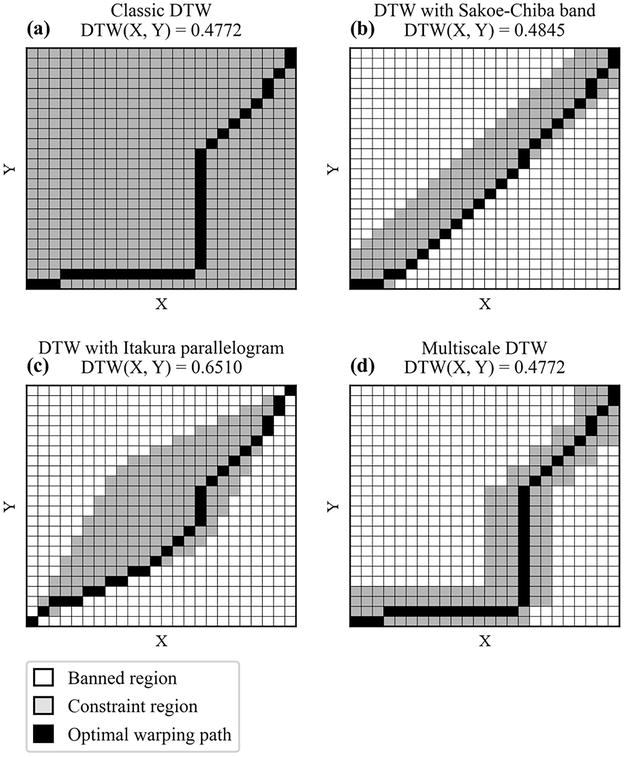
\includegraphics[width=0.5\linewidth]{dissertation//figures/dtw.png}
    \caption{Representations of various optimisation to the DTW algorithm\cite{faouzi2024time}}
    \label{fig:dtw}
\end{figure}

FastDTW looks to accelerate DTW by reducing the resolution of the matrix and gradually increasing it to give an accurate estimation\cite{salvador2007toward}. The time series are reduced in size by combining values, which leads to a smaller matrix and easier computing. The warped path from this matrix can then be used to exclude sections of the matrix in higher resolutions. Eventually, the full warped path through the full-resolution matrix is computed but with a significant proportion of the matrix removed. This is illustrated by Figure \ref{fig:fast-dtw}.

\begin{figure}[h]
    \centering
    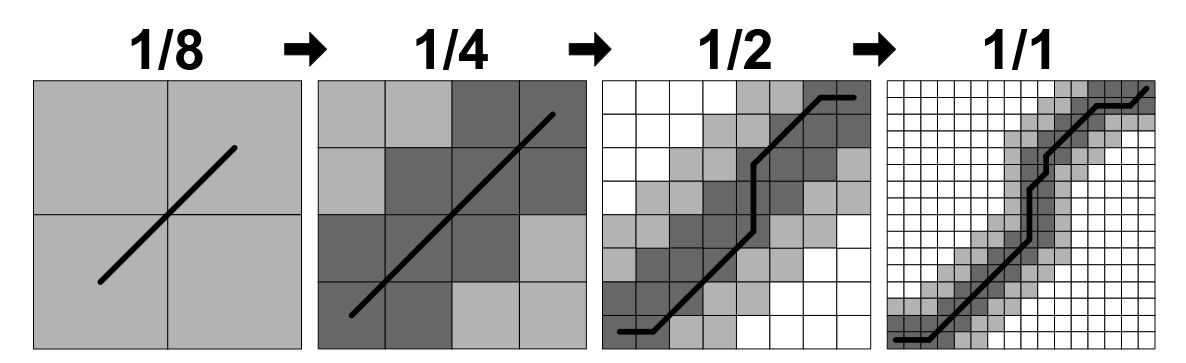
\includegraphics[width=0.75\linewidth]{dissertation//figures/fast-dtw.png}
    \caption{A representation of the different resolutions computed for FastDTW and how they exclude regions of the cost matrix in finer resolution\cite{salvador2007toward}}.
    \label{fig:fast-dtw}
\end{figure}

Whilst k-NN can be done for any value $k$, it is common to use 1-NN when dealing with time series classification.

DTW is useful for blink-based DeepFake detection as humans do not blink in unison and hence blinks will appear at seemingly random intervals in the time series. This would cause a traditional distance-based k-NN but would be correctly handled by DTW, resulting in more accurate DeepFake detection.

\subsubsection{Learning Shapelets}

Shapelets are defined as ``a subsequence of consecutive observations from a time series"\cite{faouzi2024time}. These can be used to get a sense of the building blocks of a time series and enable classification based on fundamental features. Learning shapelets\cite{grabocka2014learning} is a modification of conventional shapelet classification by optimising shapelets during training. 

First $k$ shapelets of length $l$ are generated randomly. Let $S = (s_1,\dots,s_l)$ be the shapelet and $T=(t_1,\dots,t_l$ be a time series. The ``distance" between the time series and the shapelet is defined in Equation\ref{eq:shapelet-distance}, note the use of Log Sum Exponent function (Equation \ref{eq:soft-min}) instead of a minimum function to make Equation \ref{eq:shapelet-distance} differentiable.

\begin{align}
    d(S,T) &= \min_{j \in \{0,\dots,n-l\}} \sum^l_{i=1} (s_i -x_{j+i})^2 \label{eq:shapelet-distance}\\
    \min_j a_j &\approx -\frac{1}{\beta} \log \sum_j e^{-\beta a_j} \label{eq:soft-min}
\end{align}

A time series can then go under a change of basis to represent them as a feature vector of the distance between it and each of the $k$ shapelets. Hence, $T$ can be represented as $(d(S_1,T),\dots,d(S_k,T))$. The new feature vector can now be used in a conventional classifier, such as logistic regression\cite{cramer2002origins}. 

Whilst the initial shapelets are random and are therefore likely to be ineffective, they can be learned. Both the distance function and logistic regression are differentiable and so can be learned via SGD\cite{robbins1951stochastic}. This can form shapelets into effective dataset discriminators.

In this case, one shapelet might be the EAR over the course of a normal blink. DeepFakes cannot simulate a blink well and might close the eye too fast or too slow, which learning shapelets may be able to pick up on to classify videos.

\subsubsection{Time Series Forest}

Many algorithms based on decision trees have been proposed for time series classification. Time series forest\cite{deng2013time} is one such algorithm. Random intervals of a minimum length are extracted from the same locations in each time series (Figure \ref{fig:time-series-forest}a). From these intervals, the mean, standard deviation, and gradient (slope) are extracted as feature vectors (Figure \ref{fig:time-series-forest}b).

\begin{figure}[h]
    \centering
    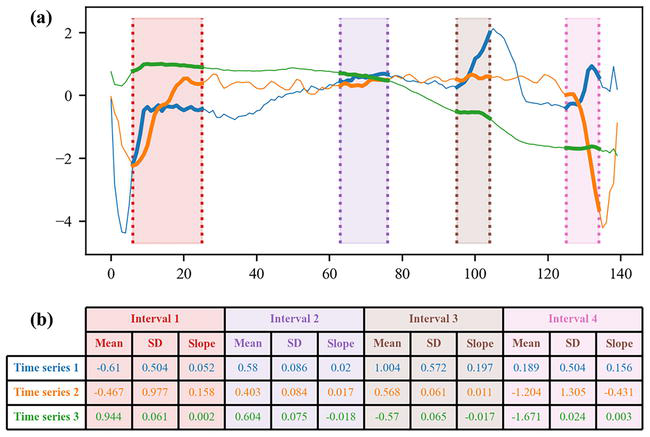
\includegraphics[width=0.5\linewidth]{dissertation//figures/time-series-forest.png}
    \caption{An example of the sequences and features extracted during the time series forest algorithm}
    \label{fig:time-series-forest}
\end{figure}

These are then fed into a forest of decision trees\cite{breiman2001random}. Decision trees are binary trees where at each node a field is compared to a value, if it is greater than a value it goes to the left child, otherwise to the right child. This continues until a leaf node, whose value acts as the final classification. A forest of decision trees processes similar data through a number of different decision trees with the final classification being the majority vote. In this case, each tree corresponds to a different interval of the time series.

Decision trees are trained from the root down. For each feature and every value in the test dataset, the dataset is split using the feature and threshold. Each split is then evaluated via a split metric function (for classification this is usually entropy). The best feature and corresponding threshold are then set for the node and the data is split. The process repeats recursively for each node until some stopping factor is reached. Stopping factors act to limit the size of tree, preventing overfitting. Common stopping factors are the depth of the tree or the minimum samples a node can contain. If a leaf node contains multiple classes from the test dataset, the class of the node is decided by a majority vote.

\subsubsection{Time Series Bag-of-Features}

Similar to a time series forest, time series bag-of-features\cite{baydogan2013bag} extracts random intervals of a minimum length from a time series. However, each interval is further split into 3 equal intervals, the mean, gradient, and standard deviation of these sub-intervals plus the interval as a whole are calculated.

Two forests are trained in this algorithm. The first is a regression tree which rather than outputting the class of an item, outputs the probability of it being in a class, taken by the number of members of each class in a leaf node. Each tree in a forest is trained on a separate subsequence. To make the probabilities more reliable a subsequence is then classified by one it was not trained on and the entire interval has its probabilities averaged across its subsequences. 

The result is for each time series, there is a set of features containing the average probability for each class and the actual probabilities of each class. These features are used as the training dataset for a second random forest which produces the final classification. 

\subsubsection{Neural Networks}
\label{sec:ts-nns}

Given the versatility of neural networks, it is unsurprising that several architectures have been proposed for time series classification. 

Intuitively, RNNs offer ideal performance as they are designed to work on temporal structures. Most RNN architectures proposed focus on LSTM modules\cite{karim2017lstm}. The architecture used for this project is a hybrid LSTM-FCN approach proposed by Karim et al\cite{karim2017lstm}. One branch of the network is a single LSTM module which can either be a standard LSTM module or an attention-LSTM module. The other branch is a standard one-dimension CNN. One-dimension CNNs are similar to their two-dimension counterparts but rather than the filter being a two-dimensional matrix, it is a one-dimensional sliding window. The results from the LSTM and CNN branches are then concatenated and fed into a single dense softmax classifier.

A number of conventional CNNs have been proposed for time series classification. A comprehensive overview is provided by Fawaz\cite{fawaz2020deep}. They propose several separate architectures, whilst the majority are for multivariate time series, some can be narrowed down to work on univariate time series. 

The first model is an MLP to act as a baseline. The architecture contains three fully connected hidden layers. The only addition is dropout layers which regulate overfitting by removing neurons randomly from a layer (typically between 10\% and 15\%). Secondly, Fawaz proposes a CNN with three convolution layers, each performing a linear transformation on the time series. A final global average pooling is used before the final dense classification to allow for time series of varying lengths to use the same architecture, however, this is not used in this project as outlined in Section \ref{sec:ts-implementation}. Time-CNN is a typical CNN for classification apart from it using mean squared error as the loss function during training instead of categorical cross entropy which is the usual loss function for classification tasks. Time series class boundaries are able to be not as distinct as other boundaries so mean squared error allows for ``smoother" classifications during training, potentially improving accuracy. The final model proposed for univariate time series is a model based on ResNet, including residual layers to improve classification.

Architectures for the above models are shown in Appendix \ref{ch:series-architectures}.

\subsubsection{Implementation}
\label{sec:ts-implementation}

The \verb|pyts| library\cite{faouzi2020pyts} is an open-source library which implements a variety of classical time series classification methods, including all the methods mentioned in this project. The CNNs proposed in Section \ref{sec:ts-nns} by Fawaz have had their architectures and training parameters open-sourced in a companion GitHub repository\cite{fawaz2019deep}. The LSTM architecture was implemented using the description from the corresponding paper. The number of epochs for LSTM was reduced from 2000 to 500 to reduce overfitting. Apart from this, all hyperparameters were left as the default values from their respective implementations.

Some of the neural network architectures require a fixed input length. To reduce computation time it was therefore decided to crop or pad all time series to 512 values. Assuming a video runs at 30 frames per second, 17 seconds of footage can be analysed, giving an ample number of blinks to be analysed. If a video has less than 512 frames, the EAR is padded with -1s at the end.

To train the models, every video in the train set is analysed by one of the facial landmark models (Section \ref{sec:eye-landmark}) to produce the EAR graph for that video. It is assumed that the train set being given to this section is balanced between real and fake videos. The graphs are then further split into a train and test set with 80\% being used for training and 20\% for testing. Models are then trained on the train set and then compared to each other on the test set. The model with the greatest accuracy is then selected as the best EAR analyser for the specific model on the specific dataset.

\section{Adversarial Noise}
\label{sec:ad-noise}

% \begin{itemize}
%     \item foolbox library (Targeted FGSM using the other thing)
%     \item chosen over cleverhans as cleverhans had meh documentation
%     \item cw-l2 attack too slow (3hrs per video)
%     \item fakeretouch has no open-source implementation, timings were too slow, estimated would also take a while
% \end{itemize}

There are two popular libraries for adding adversarial noise: \verb|foolbox|\cite{rauber2017foolbox}\cite{rauber2017foolboxnative} and \verb|cleverhans|\cite{papernot2018cleverhans}. Both offer similar feature sets with native support for TensorFlow, a wide variety of documentation and open-source code bases. Hence, any choice between is based on preference rather than an objective view. \verb|foolbox| was chosen as the library for adversarial noise as it was the most up-to-date library. Furthermore, a bug in \verb|cleverhans|' source code meant the auto-generated documentation appeared blank and so had to be inferred by looking at the source code. On the other hand, \verb|foolbox| had a much richer and working documentation site, allowing for easier bug fixing if necessary.

Whilst \verb|foolbox| does have an implementation of FGSM, it is an untargeted attack in their implementation. As a result, the attack is less reliable than the targeted attack proposed by Gandhi et al.\cite{gandhi2020adversarial}. To target the FGSM attack using \verb|foolbox|, a Projected Gradient Descent attack with 1 step in its search can be used\cite{madry2017towards}. This is an equivalent attack and as such can be introduced without loss of generality.

The CW-L2 attack proved to be too slow for videos. To attack a video, FGSM took 10 seconds, whereas the CW-L2 attack to 3 hours on the same hardware and video. The majority of video-based DeepFake detection datasets contain thousands of videos. As such, the CW-L2 attack was not tested in this project due to time constraints.

Finally, FakeRetouch comes with no open-source code implementation. Following the delay caused by the failed implementation of WSELD due to its lack of implementation, there was little time available for further development work. Therefore, no evaluation was done on FakeRetouch. The reasons for this choice are explained in greater detail in Chapter \ref{ch:projman}.

\section{Traditional Detectors}
\label{sec:traditional-detectors}

The VGG19\cite{krishna2022deepfake}\cite{yadav2024deepfake} and ResNet\cite{tiwari2024deepfake} models from the proof of concept are used in the main algorithm loop. Additional state-of-the-art DeepFake detectors have been created to evaluate their performance against adversarial noise. State-of-the-detectors were taken as the best performing DeepFake detection models uploaded to the PapersWithCode leaderboard\footnote{\url{https://paperswithcode.com/sota/deepfake-detection-on-faceforensics}}\footnote{\url{https://paperswithcode.com/sota/deepfake-detection-on-faceforensics-1}} that had open-source repositories. The models chosen were based on EfficinetNetB4\cite{bonettini2021video} and Xception\cite{roessler2019faceforensicspp}.

EfficientNetB4 was chosen from the EfficinetNet family of models by Bonettini et al. due to its balance between the number of parameters, run time, and classification performance. Two models based on EfficientNet are proposed in the paper, one using the standard EfficientNet and another with an attention module added. These were shown to have very similar results so, to keep the network architecture simple, just EfficientNetB4 is used as the backbone with no attention model added.

Xception was chosen by R\"{o}ssler et al for classification from a pool of four other CNNs. When compared to the other CNNs, Xception proved to be the most accurate at 99.26\% accuracy.

Custom headers were added to these backbones to allow for accurate classification. Firstly, the networks are stripped of their initial classification heads to allow fine tuning on DeepFakes. Secondly, global pooling reduces the high dimension features outputted from the backbone into a single one dimensional vector. The resulting vector is then normalised to allow for quicker and easier training. To reduce overfitting, a dropout layer is added to reduce the size of the final vector by 50\%. Finally, a dense layer produces the final classification.

Model diagrams of the CNNs used for classifications can be found in Appendix \ref{ch:trad-architectures}.

The training dataset for these CNNs is created by splitting the overall training set into 80\% for model training, and 20\% for model validation. For every video in the model training set, 32 frames are extracted and cropped to the facial region, following the method to train EfficientNet\cite{bonettini2021video}. To prevent overfitting, it is important for frames in the same video to not be used in both the training set and validation set, a phenomenon referred to as data leakage. Similarly to the proof of concept, no videos that have adversarial noise added to them are used in the training data as this would not reflect the scenarios DeepFake detectors would see in real life.

When training, models are trained using categorical cross-entropy. The Adam\cite{kingma2014adam} optimiser is used for optimising gradients with hyperparameters from the original paper's implementations. Models were trained for 20 epochs, however early stopping was implemented to reduce the time to learn and to reduce overfitting. If a model's validation loss stops improving for 5 consecutive epochs, training is halted. To further reduce overfitting, the learning rate of the Adam optimiser is reduced by 90\% if the validation loss does not improve for 3 consecutive epochs. To gain the benefits of transfer learning, all models were initialised with their weights from the ImageNet\cite{deng2009imagenet} dataset.

When classifying a video, each frame is independently classified by the model. If more than 50\% of the frames in a video are reported fake, then the video is deemed a fake. This threshold was chosen over a static threshold to account for varying length videos. 50\% was chosen as the threshold as it means the majority of frames needed to be classified fake for a video to be fake. One potential concern is uncertain predictions which could cause the model to predict randomly, therefore causing false classifications. However, when testing on images, the model was often confident in its output, often outputting probabilities close to 1 for the chosen classification. 

\section{Final Code}

% \begin{itemize}
%     \item One codebase to do full training, splitting and evaluation
%     \item just give overall flow diagram?
%     \item {\huge models only trained on non-noisy images}
%     \item checkpointing where possible
%     \item run on either dcs compute clusters or avon
%     \item final speeds + hardware
% \end{itemize}

To make final testing and evaluation easier, it was decided to centralise the code for this project in one main loop. One piece of code, upon given a dataset and facial landmarking model, would train all other models required, and evaluate them. Facial landmarking models are trained separately as these require a different dataset for training and are invariant across datasets and therefore training them in the main program would be inefficient.

The program structure is shown in Algorithm \ref{alg:final-code}.

\begin{algorithm}[H]
    \caption{Final Code}
    \label{alg:final-code}
    \begin{algorithmic}
        \Require dataset, \textsc{FaceLandmarks} \Comment{dataset and facial landmarker function call}

        \State train\_set, test\_set $\gets$ \textsc{SplitDataset}(dataset)
        \State \textsc{CustomAnalyser} $\gets$ \textsc{GetBestAnalyser}(train\_set, \textsc{FaceLandmarks})
        \State \textsc{TraiditionalModels} $\gets$ \textsc{GetModels}(train\_set)
        \For{video, label $\in$ test\_set}
            \State landmarks $\gets$ \{\}
            \State model\_predictions $\gets$ \{\}
            \State noisy\_landmarks $\gets$ \{\}
            \State noisy\_model\_predictions $\gets$ \{\}
            \For{frame $\in$ video}
                \State \textsc{Append}(landmarks, \textsc{FaceLandmarks}(frame))
                \State \textsc{Append}(model\_predictions, \textsc{TraditionalModels}(frame))
                \If{label = FAKE}
                    \State noisy\_frames $\gets$ \textsc{AttackFrame}(frame, \textsc{TraditionalModels})
                    \State \textsc{Append}(noisy\_landmarks, \textsc{FaceLandmarks}(noisy\_frames))
                    \State \textsc{Append}(noisy\_model\_predictions, \textsc{TraditionalModels}(noisy\_frames))
                \Else
                    \State \textsc{Append}(noisy\_landmarks, \textsc{FaceLandmarks}(frame))
                    \State \textsc{Append}(noisy\_model\_predictions, \textsc{TraditionalModels}(frame))
                \EndIf
            \EndFor 
            \State traditional\_classifications $\gets$ \textsc{ClassifyVideosClassical}(model\_predictions)
            \State noisy\_traditional\_classifications $\gets$ \textsc{ClassifyVideosClassical}(noisy\_model\_predictions)
            \State custom\_classifications $\gets$ \textsc{CustomAnalyser}(landmarks)
            \State noisy\_custom\_classifications $\gets$ \textsc{CustomAnalyser}(noisy\_landmarks)
        \EndFor
    \end{algorithmic}
\end{algorithm}

Often with DeepFake datasets, multiple DeepFake videos are generated from a single real video. As such, there are often more fake videos than real ones. This can cause issues when training as a model could achieve a high accuracy by simply predicting fake every time. To ensure an even split, the dataset is split according to the number of real videos in the dataset. 80\% of the real videos are taken for training, the same number of fake videos are then used in the train set for an even split. The remaining videos are used for the testing set. Note that the train set is further split into a training set and validation set in the \textsc{GetBestAnalyser} and \textsc{GetModels} functions as outlined in Sections \ref{sec:ts-implementation} and \ref{sec:traditional-detectors}.

Frames are only attacked if they are fake frames as this reflects reality where an adversary would only add noise to a video if the video was faked. This also has the advantage of significantly reducing compute times as not only is attacking the frame skipped, but classifying each attacked frame with every model is avoided as well. \verb|noisy_frames| is a tuple of 4 frames, each frame attacking a single one of the traditional models. 

In line with good scientific computing practices, the main code has checkpoints. All models trained are saved so that they can be retrieved should the program ever terminate. The path to the best model selected by \textsc{GetBestAnalyser} is also saved so that all the models do not have to be re-evaluated. Every 25 videos, the ongoing results of the main video loop are saved so in the event the main loop crashes or is timed out, the loop can pick up from where it last saved.

\section{Transferability}

To evaluate the transferability of blink-based DeepFake detection, the FakeAVCeleb dataset from Section \ref{sec:datasets} will be reserved. As such, no model shall be trained on FakeAVCeleb. The main program will be run across all datasets which will produce models that have been trained on each of the other datasets. All of the traditional models and each of the custom models will then be tested on the FakeAVCeleb dataset. To save time and compute resources, only the eye landmarked and associated best EAR analysis model for the dataset it was trained on will be used to evaluate transferability.

The testing algorithm follows the same rough structure as Algorithm \ref{alg:final-code}, with three main differences. The dataset is not split into a train and a test set as the entire dataset is used for testing. Secondly, all the models are loaded as they have already been trained. In the main classification loop, no adversarial noise is added to the frames, hence the \verb|noisy_*| result stores are omitted along with the calls to \textsc{AttackFrame}. Similar to the main code loop, the results are saved every 25 videos to be able to recover from crashes and other associated errors. 

\section{Datasets}

An attempt was made to access all of the datasets listed in Section \ref{sec:datasets}. For the majority of them, the application involved filling in a form and agreeing to each dataset's respective terms and conditions. However, gaining access to the DFDC dataset\cite{dolhansky2020deepfake} proved difficult. The original Kaggle competition the dataset was posted under\footnote{\url{https://www.kaggle.com/competitions/deepfake-detection-challenge}} has closed and hence it is impossible to download the dataset from that source. From the DFDC's website, the dataset should be available at \url{https://dfdc.ai/}, however, the site known longer has a valid SSL certificate (Appendix \ref{ch:dfdcai}) and can therefore not be accessed securely. The website requires a username, password, and Amazon Web Service account ID. Some of this is sensitive information and is therefore unadvisable to upload over an insecure connection. As a result, testing on the DFDC is not completed in this project.

All datasets were downloaded from their original source. FaceForensics has the option to be downloaded at multiple compression levels, to balance disk space and quality, the middle compression level (c23) was chosen.